% ===================================================================
%  Week 12 — Session 2: Training, evaluation & the limits of features
% ===================================================================
\documentclass[10pt,aspectratio=169]{beamer}
% ===================================================================
%  Shared Beamer preamble for "Practical Image Processing"
%  English slides. Compile with pdfLaTeX.
% ===================================================================

\usetheme{metropolis}
\usepackage[T1]{fontenc}
\usepackage[utf8]{inputenc}
\usepackage{lmodern}
\usepackage{listings}
\usepackage{tcolorbox}
\usepackage{fontawesome5}
\usepackage{booktabs}
\usepackage{amsmath,amssymb}
\usepackage{tikz}
\usepackage{pgfplots}
\pgfplotsset{compat=1.17}
\usetikzlibrary{arrows.meta,positioning,shapes.geometric,fit,backgrounds,matrix}
\tcbuselibrary{skins,breakable}

% ---- Palette --------------------------------------------------------
\definecolor{coursePrimary}{HTML}{1B4965}   % deep blue
\definecolor{courseAccent}{HTML}{E76F51}    % coral
\definecolor{courseGood}{HTML}{2A9D8F}      % teal
\definecolor{courseBad}{HTML}{C0392B}       % red
\definecolor{courseInfo}{HTML}{2980B9}      % blue
\definecolor{codeBg}{HTML}{F5F6FA}
\definecolor{codeKw}{HTML}{8E44AD}
\definecolor{codeStr}{HTML}{2A9D8F}
\definecolor{codeCom}{HTML}{7F8C8D}

\setbeamercolor{frametitle}{bg=coursePrimary}
\setbeamercolor{progress bar}{fg=courseAccent}
\setbeamercolor{alerted text}{fg=courseAccent}
\metroset{block=fill,sectionpage=progressbar,numbering=fraction}

% ---- Code listings (Python is built into listings) -----------------
\lstdefinestyle{course}{
  backgroundcolor=\color{codeBg},
  basicstyle=\ttfamily\scriptsize,
  keywordstyle=\color{codeKw}\bfseries,
  stringstyle=\color{codeStr},
  commentstyle=\color{codeCom}\itshape,
  numberstyle=\tiny\color{codeCom},
  numbers=left, numbersep=6pt,
  showstringspaces=false, breaklines=true, breakatwhitespace=true,
  tabsize=4, columns=fullflexible,
  frame=single, framesep=4pt, rulecolor=\color{gray!30},
  keepspaces=true, upquote=true, language=Python,
}
\lstset{style=course}
\lstdefinelanguage{bash}{
  keywords={cd,pip,python,venv,source,import}, sensitive=true,
  morecomment=[l]{\#}, morestring=[b]', morestring=[b]",
}

% ---- Reusable callout boxes ----------------------------------------
\newtcolorbox{goodbox}[1][Good practice]{colback=courseGood!8,colframe=courseGood,
  fonttitle=\bfseries,title={\faCheck~#1},boxrule=0.6pt,left=4pt,right=4pt,top=3pt,bottom=3pt}
\newtcolorbox{badbox}[1][Pitfall]{colback=courseBad!8,colframe=courseBad,
  fonttitle=\bfseries,title={\faTimes~#1},boxrule=0.6pt,left=4pt,right=4pt,top=3pt,bottom=3pt}
\newtcolorbox{infobox}[1][Note]{colback=courseInfo!8,colframe=courseInfo,
  fonttitle=\bfseries,title={\faInfoCircle~#1},boxrule=0.6pt,left=4pt,right=4pt,top=3pt,bottom=3pt}
\newtcolorbox{mathbox}[1][Math]{colback=coursePrimary!6,colframe=coursePrimary,
  fonttitle=\bfseries,title={\faCalculator~#1},boxrule=0.6pt,left=4pt,right=4pt,top=3pt,bottom=3pt}

\newcommand{\keyidea}[1]{\begin{alertblock}{Key idea}#1\end{alertblock}}
\newcommand{\term}[1]{\textbf{\color{coursePrimary}#1}}
\newcommand{\code}[1]{\lstinline[basicstyle=\ttfamily\small]|#1|}

% ---- A helper to draw a small pixel grid, cells shaded by value ----
% \pixelgrid{ {10,20,120,200,240}, {30,60,130,180,230}, ... }
\newcommand{\pixelgrid}[1]{%
  \begin{tikzpicture}[font=\scriptsize,scale=0.6]
    \foreach \row [count=\ry] in {#1} {
      \foreach \val [count=\cx] in \row {
        \draw[gray,fill=coursePrimary!8] (\cx,-\ry) rectangle ++(1,-1);
        \node at (\cx+0.5,-\ry-0.5) {\val};
      }
    }
  \end{tikzpicture}}


\title{From Features to Machine Learning}
\subtitle{Week 12 — Session 2: Training, evaluation \& the limits of hand-crafted features}
\author{Practical Image Processing}
\date{Lecture 12.2 \textbullet\ 60--70 min}

\begin{document}

\maketitle

\begin{frame}{Recap of Session 1}
  \begin{columns}[T]
    \begin{column}{0.58\textwidth}
      \begin{itemize}
        \item We turn an image into a compact \term{feature vector} (HOG $+$ optionally colour).
        \item HOG histograms gradient \emph{orientations} per cell — a robust shape signature.
        \item A \term{classifier} (k-NN, SVM) learns a boundary in that feature space.
        \item We set up a \term{stratified} 70/30 train/test split.
      \end{itemize}
    \end{column}
    \begin{column}{0.42\textwidth}
      \begin{alertblock}{Today}
        Train the classifiers, measure them \emph{honestly}, and confront overfitting on look-alike cars.
      \end{alertblock}
    \end{column}
  \end{columns}
\end{frame}

\begin{frame}{Roadmap}\tableofcontents\end{frame}

% ==================================================================
\section{Training the classifier}
% ==================================================================

\begin{frame}[fragile]{The whole ML pipeline in code}
\begin{lstlisting}[language=Python]
X = [hog(gray(img)) for img in images]      # features
Xtr, Xte, ytr, yte = train_test_split(X, y, test_size=0.3,
                                      stratify=y)
clf = SVC(kernel='rbf', C=10).fit(Xtr, ytr) # learn
print(accuracy_score(yte, clf.predict(Xte)))# HONEST score
print(confusion_matrix(yte, clf.predict(Xte)))
\end{lstlisting}
  Extract features $\rightarrow$ split $\rightarrow$ fit $\rightarrow$ evaluate on unseen data. Always in that order.
\end{frame}

\begin{frame}[fragile]{Building $X$ and $y$ from your images}
\begin{lstlisting}[language=Python]
from skimage.feature import hog
import cv2, numpy as np

def features(path):
    g = cv2.cvtColor(cv2.imread(path), cv2.COLOR_BGR2GRAY)
    g = cv2.resize(g, (96, 96))
    return hog(g, pixels_per_cell=(8,8), cells_per_block=(2,2),
               orientations=9)

X = np.array([features(p) for p in paths])   # (N, ~900)
y = np.array(labels)                         # 0=206,1=405,2=Dena
\end{lstlisting}
  Every image becomes one row of $X$; \code{y} holds its class. Resize first so all vectors are the same length.
\end{frame}

\begin{frame}[fragile]{Fitting both classifiers}
\begin{lstlisting}[language=Python]
from sklearn.neighbors import KNeighborsClassifier
from sklearn.svm import SVC
from sklearn.preprocessing import StandardScaler
from sklearn.pipeline import make_pipeline

knn = make_pipeline(StandardScaler(),
                    KNeighborsClassifier(n_neighbors=5))
svm = make_pipeline(StandardScaler(),
                    SVC(kernel='rbf', C=10))
knn.fit(Xtr, ytr);  svm.fit(Xtr, ytr)
\end{lstlisting}
  \begin{goodbox}
    Wrapping the scaler in a \code{Pipeline} means it is fit on training folds only — no leakage into the test set.
  \end{goodbox}
\end{frame}

% ==================================================================
\section{Evaluating honestly}
% ==================================================================

\begin{frame}{Our real results (and an honest lesson)}
  \begin{center}
  \begin{tabular}{@{}lcc@{}}
    \toprule
    \textbf{Classifier} & \textbf{Train acc} & \textbf{Test acc} \\
    \midrule
    k-NN ($k{=}5$) & 0.65 & 0.43 \\
    SVM (RBF) & \alert{1.00} & \alert{0.48} \\
    \bottomrule
  \end{tabular}
  \end{center}
  \vspace{3pt}
  Chance is 0.33 (3 classes). Both beat chance — but the SVM scores \textbf{100\% on train, 48\% on test}.
  That gap is \term{overfitting}.
\end{frame}

\begin{frame}{Overfitting, explained}
  \begin{itemize}
    \item \term{Overfitting}: the model memorizes training quirks instead of the real pattern.
    \item Symptom: train accuracy $\gg$ test accuracy (here 1.00 vs 0.48).
    \item Cures: more data, simpler model, regularization, better/invariant features.
  \end{itemize}
  \keyidea{A model that is perfect on training data and mediocre on test data has learned the wrong thing.}
\end{frame}

\begin{frame}{Why our SVM overfit so hard}
  \begin{itemize}
    \item Only 126 training vectors, each 900-dimensional — far more features than examples.
    \item An RBF SVM with high $C$ can bend the boundary to fit every training point exactly.
    \item Result: train 1.00, but the boundary is tuned to noise $\rightarrow$ test collapses to 0.48.
  \end{itemize}
  \keyidea{More dimensions than samples is a red flag: the model has enough freedom to memorize. Reduce $C$, reduce dimensions (PCA), or get more data.}
\end{frame}

\begin{frame}{The bias--variance tradeoff}
  \begin{columns}[T]
    \begin{column}{0.5\textwidth}
      \begin{center}
      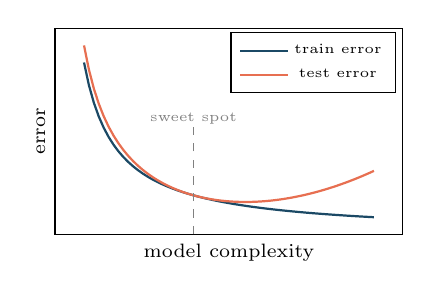
\begin{tikzpicture}
        \begin{axis}[width=6cm,height=4.2cm,
            xlabel={\scriptsize model complexity},ylabel={\scriptsize error},
            xlabel style={font=\scriptsize},ylabel style={font=\scriptsize},
            xtick=\empty,ytick=\empty,legend style={font=\tiny,at={(0.98,0.98)},anchor=north east},
            domain=0.5:5,samples=60]
          \addplot[coursePrimary,thick] {1.6/x};
          \addlegendentry{train error}
          \addplot[courseAccent,thick] {1.6/x + 0.11*(x-2.2)^2};
          \addlegendentry{test error}
          \draw[dashed,gray] (axis cs:2.2,0) -- (axis cs:2.2,2);
          \node[gray,font=\tiny] at (axis cs:2.2,2.15) {sweet spot};
        \end{axis}
      \end{tikzpicture}
      \end{center}
    \end{column}
    \begin{column}{0.5\textwidth}
      \begin{itemize}
        \item Too simple $\Rightarrow$ high \term{bias}: underfits, both errors high.
        \item Too complex $\Rightarrow$ high \term{variance}: overfits, test error climbs back up.
        \item Our RBF SVM sits far to the right: train error $0$, test error large.
      \end{itemize}
    \end{column}
  \end{columns}
\end{frame}

\begin{frame}{Reading the confusion matrix}
  \begin{columns}[T]
    \begin{column}{0.5\textwidth}\begin{center}
      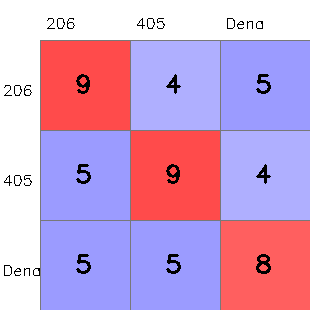
\includegraphics[width=0.95\linewidth]{../assets/confusion.png}
    \end{center}\end{column}
    \begin{column}{0.5\textwidth}
      \begin{itemize}
        \item Rows = true class, columns = predicted.
        \item Diagonal = correct; off-diagonal = the mistakes.
        \item Shows \emph{which} models get confused — far more useful than a single accuracy number.
      \end{itemize}
    \end{column}
  \end{columns}
\end{frame}

\begin{frame}{Confusion matrix — working the numbers}
  \begin{columns}[T]
    \begin{column}{0.5\textwidth}
      A $3$-class test set (rows $=$ true, cols $=$ predicted):
      \begin{center}
      \begin{tabular}{@{}l|ccc@{}}
        \toprule
         & \small 206 & \small 405 & \small Dena \\
        \midrule
        \small 206  & \textbf{8} & 3 & 1 \\
        \small 405  & 4 & \textbf{6} & 2 \\
        \small Dena & 2 & 3 & \textbf{7} \\
        \bottomrule
      \end{tabular}
      \end{center}
    \end{column}
    \begin{column}{0.5\textwidth}
      For class \term{206}:
      \begin{mathbox}
        $TP=8,\ FP=4{+}2=6,\ FN=3{+}1=4$.\\[3pt]
        Precision $=\tfrac{8}{8+6}=0.57$.\\[2pt]
        Recall $=\tfrac{8}{8+4}=0.67$.
      \end{mathbox}
      206 is most confused with 405 ($3$ and $4$ off-diagonal both ways).
    \end{column}
  \end{columns}
\end{frame}

\begin{frame}{Metrics beyond accuracy}
  \begin{itemize}
    \item \term{Accuracy} hides imbalance: 95\% ``all normal'' is useless if 5\% are the faults you need.
    \item \term{Precision}: of predicted-positive, how many were right? \term{Recall}: of actual-positive, how many did we catch?
    \item \term{F1}: their harmonic mean. Report these per class, not one global number.
  \end{itemize}
  \begin{mathbox}
    Precision $=\dfrac{TP}{TP+FP}$,\quad Recall $=\dfrac{TP}{TP+FN}$,\quad F1 $=\dfrac{2\,PR}{P+R}$.
  \end{mathbox}
\end{frame}

\begin{frame}{Precision vs recall — a worked tradeoff}
  \begin{columns}[T]
    \begin{column}{0.55\textwidth}
      A fault detector on 100 parts (4 truly faulty):
      \begin{itemize}
        \item ``Always OK'' $\Rightarrow$ accuracy $96\%$, but recall on faults $=0$. Useless.
        \item Flag anything suspicious $\Rightarrow$ recall $\uparrow$, precision $\downarrow$ (many false alarms).
      \end{itemize}
    \end{column}
    \begin{column}{0.45\textwidth}
      \begin{mathbox}
        Catch $3/4$ faults but raise $6$ false alarms:\\[3pt]
        Precision $=\tfrac{3}{3+6}=0.33$,\\[2pt]
        Recall $=\tfrac{3}{4}=0.75$,\\[2pt]
        F1 $=\tfrac{2\cdot0.33\cdot0.75}{0.33+0.75}\approx 0.46$.
      \end{mathbox}
    \end{column}
  \end{columns}
  \keyidea{Which matters more depends on the cost: missing a fault vs raising a false alarm.}
\end{frame}

% ==================================================================
\section{Doing it right}
% ==================================================================

\begin{frame}{Cross-validation \& not fooling yourself}
  \begin{itemize}
    \item A single split is noisy. \term{k-fold cross-validation} averages over $k$ splits for a stable estimate.
    \item Tune hyper-parameters on a \term{validation} set (or CV) — never on the test set.
    \item The test set is used \emph{once}, at the very end. Peeking at it inflates your reported score.
  \end{itemize}
\end{frame}

\begin{frame}{k-fold cross-validation, illustrated}
  \begin{columns}[T]
    \begin{column}{0.56\textwidth}
      \begin{center}
      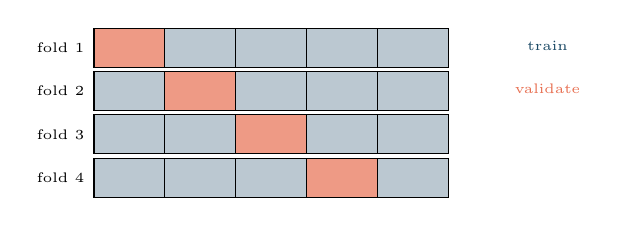
\begin{tikzpicture}[font=\tiny,x=0.9cm,y=0.55cm]
        \foreach \r in {0,1,2,3}{
          \foreach \c in {0,1,2,3,4}{
            \ifnum\c=\r
              \fill[courseAccent!70] (\c,-\r) rectangle ++(1,-0.9);
            \else
              \fill[coursePrimary!30] (\c,-\r) rectangle ++(1,-0.9);
            \fi
            \draw (\c,-\r) rectangle ++(1,-0.9);
          }
          \node[left] at (0,-\r-0.45) {fold \the\numexpr\r+1\relax};
        }
        \node[courseAccent] at (6.4,-1.4) {validate};
        \node[coursePrimary] at (6.4,-0.4) {train};
      \end{tikzpicture}
      \end{center}
    \end{column}
    \begin{column}{0.44\textwidth}
      \begin{itemize}
        \item Split data into $k$ folds (here $k{=}5$, one row shown per fold used for validation).
        \item Each fold serves once as validation, $k{-}1$ times for training.
        \item Average the $k$ scores $\Rightarrow$ a stable estimate with less luck.
      \end{itemize}
    \end{column}
  \end{columns}
\end{frame}

\begin{frame}[fragile]{Hyper-parameter tuning with grid search}
\begin{lstlisting}[language=Python]
from sklearn.model_selection import GridSearchCV
grid = {'svc__C': [0.1, 1, 10, 100],
        'svc__gamma': ['scale', 0.01, 0.001]}
gs = GridSearchCV(svm, grid, cv=5)   # 5-fold CV inside train
gs.fit(Xtr, ytr)
print(gs.best_params_)               # chosen WITHOUT the test set
print(gs.score(Xte, yte))            # test used ONCE, at the end
\end{lstlisting}
  \begin{badbox}
    Never put \code{Xte} inside \code{GridSearchCV}. Tuning on the test set is how honest projects quietly cheat.
  \end{badbox}
\end{frame}

\begin{frame}{Regularization: the $C$ knob}
  \begin{columns}[T]
    \begin{column}{0.5\textwidth}
      \begin{center}
      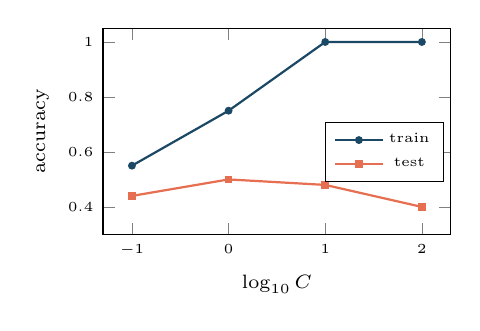
\begin{tikzpicture}
        \begin{axis}[width=6cm,height=4.2cm,
            xlabel={\scriptsize $\log_{10} C$},ylabel={\scriptsize accuracy},
            xlabel style={font=\scriptsize},ylabel style={font=\scriptsize},
            tick label style={font=\tiny},ymin=0.3,ymax=1.05,
            legend style={font=\tiny,at={(0.98,0.4)},anchor=east}]
          \addplot[coursePrimary,thick,mark=*,mark size=1pt] coordinates
            {(-1,0.55)(0,0.75)(1,1.0)(2,1.0)};
          \addlegendentry{train}
          \addplot[courseAccent,thick,mark=square*,mark size=1pt] coordinates
            {(-1,0.44)(0,0.50)(1,0.48)(2,0.40)};
          \addlegendentry{test}
        \end{axis}
      \end{tikzpicture}
      \end{center}
    \end{column}
    \begin{column}{0.5\textwidth}
      \begin{itemize}
        \item Large $C$: fit training hard $\Rightarrow$ train $\to 1.0$, test drops (overfit).
        \item Small $C$: softer margin, more errors allowed $\Rightarrow$ better generalization.
        \item Pick $C$ by cross-validation, not by the train score.
      \end{itemize}
      \begin{goodbox}
        The best test score here is at a \emph{moderate} $C$, not the largest.
      \end{goodbox}
    \end{column}
  \end{columns}
\end{frame}

% ==================================================================
\section{In-class exercise}
% ==================================================================

\begin{frame}{\faPen~In-class exercise (10 min)}
  \begin{infobox}[Diagnose the model]
  \end{infobox}
  \begin{enumerate}
    \item Our SVM got train 1.00, test 0.48. Name the problem and two ways to reduce it.
    \item A fault detector reports 96\% accuracy but faults are 4\% of data. Why might it be useless?
    \item You want to tell 206 from 405. What feature besides HOG might help separate them?
  \end{enumerate}
\end{frame}

\begin{frame}{\faPen~Debrief}
  \begin{itemize}
    \item (1) \term{Overfitting}: gather more data, simplify/regularize the SVM (lower $C$), or use better features.
    \item (2) Predicting ``no fault'' always scores 96\% but has \term{zero recall} on faults — accuracy is the wrong metric.
    \item (3) \term{Colour histograms} (models differ in typical colour), size/aspect, or logo region features.
  \end{itemize}
  \keyidea{A number without a train/test split and a confusion matrix tells you almost nothing.}
\end{frame}

% ==================================================================
\section{The limit of hand-crafted features}
% ==================================================================

\begin{frame}{Feature engineering vs feature learning}
  \begin{itemize}
    \item Today we \term{engineered} features (HOG) and learned only the classifier.
    \item The 48\% ceiling on look-alike cars hints at the limit of hand-designed features.
    \item \term{Deep learning} (Weeks 13--14) \emph{learns the features too}, directly from pixels.
  \end{itemize}
  \keyidea{The classical pipeline plateaus on hard, fine-grained problems. That plateau is exactly why CNNs took over.}
\end{frame}

\begin{frame}{The plateau of hand-crafted features}
  \begin{columns}[T]
    \begin{column}{0.5\textwidth}
      \begin{center}
      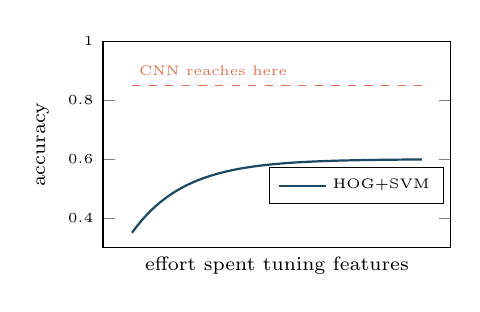
\begin{tikzpicture}
        \begin{axis}[width=6cm,height=4.2cm,
            xlabel={\scriptsize effort spent tuning features},ylabel={\scriptsize accuracy},
            xlabel style={font=\scriptsize},ylabel style={font=\scriptsize},
            xtick=\empty,ymin=0.3,ymax=1.0,tick label style={font=\tiny},
            legend style={font=\tiny,at={(0.98,0.3)},anchor=east},domain=0:5,samples=60]
          \addplot[coursePrimary,thick] {0.35+0.25*(1-exp(-1.1*x))};
          \addlegendentry{HOG+SVM}
          \draw[dashed,courseAccent] (axis cs:0,0.85) -- (axis cs:5,0.85);
          \node[courseAccent,font=\tiny] at (axis cs:1.4,0.9) {CNN reaches here};
        \end{axis}
      \end{tikzpicture}
      \end{center}
    \end{column}
    \begin{column}{0.5\textwidth}
      \begin{itemize}
        \item More feature tuning gives diminishing returns — the curve flattens.
        \item The gap to a learned representation stays open on fine-grained tasks.
        \item You cannot hand-design your way past look-alike classes.
      \end{itemize}
    \end{column}
  \end{columns}
\end{frame}

\begin{frame}{Where this fits DocScan}
  \begin{itemize}
    \item DocScan must read digits. A digit is a small image; a classifier maps it to 0--9.
    \item Today's pipeline (features $\rightarrow$ classifier) is exactly how classic OCR worked.
    \item Next week we replace hand features with a \term{CNN} that learns them — and accuracy jumps.
  \end{itemize}
\end{frame}

\begin{frame}{Toward learned features (Weeks 13--14)}
  \begin{center}
  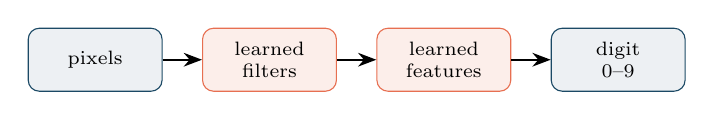
\begin{tikzpicture}[font=\scriptsize,node distance=5mm,>=Stealth,
      box/.style={draw=coursePrimary,fill=coursePrimary!8,rounded corners,
        minimum height=8mm,minimum width=17mm,align=center}]
    \node[box] (px) {pixels};
    \node[box,right=of px,fill=courseAccent!12,draw=courseAccent] (conv) {learned\\filters};
    \node[box,right=of conv,fill=courseAccent!12,draw=courseAccent] (deep) {learned\\features};
    \node[box,right=of deep] (out) {digit\\0--9};
    \draw[->,thick] (px)--(conv); \draw[->,thick] (conv)--(deep); \draw[->,thick] (deep)--(out);
  \end{tikzpicture}
  \end{center}
  \begin{itemize}
    \item A CNN replaces HOG with filters it \emph{learns} — the orange boxes are trained, not designed.
    \item Same pipeline shape as today; the difference is \emph{who} designs the features.
  \end{itemize}
\end{frame}

% ==================================================================
\section{Wrap-up \& deliverable}
% ==================================================================

\begin{frame}{What you should now be able to do}
  \begin{itemize}
    \item Build a features $\rightarrow$ classifier pipeline (HOG + SVM/k-NN) on real images.
    \item Split train/test correctly and read a confusion matrix.
    \item Recognize overfitting (train $\gg$ test) and name cures.
    \item Explain why accuracy alone misleads, and when precision/recall matter.
    \item Use cross-validation and grid search without leaking the test set.
  \end{itemize}
\end{frame}

\begin{frame}{This week's deliverable}
  \begin{alertblock}{Due before Week 13 (see \code{project/})}
    \begin{enumerate}
      \item Extract HOG features for 2--3 classes from \code{E:/data}; build $X, y$.
      \item Train k-NN and SVM with a stratified train/test split; report both accuracies.
      \item Show the confusion matrix; identify which classes get confused.
      \item Diagnose overfitting and try one cure (lower $C$, PCA, or more data); report whether the test score improved.
    \end{enumerate}
  \end{alertblock}
\end{frame}

\begin{frame}[standout]
  Features make it learnable; the split keeps you honest.\\[4pt]
  \normalsize Hand-designed features hit a ceiling — next week we learn the features themselves.
\end{frame}

\end{document}
